% -*- coding: UTF-8 -*-

\documentclass[UTF8,8pt,xcolor=dvipsnames]{beamer}

\usepackage{xeCJK}
\usepackage[utf8]{inputenc}

\usepackage{hyperref}
% \hypersetup{pdftex,colorlinks=true,allcolors=blue}
\usepackage{hypcap}

\usepackage{color}
\usepackage{xcolor}

\usepackage{amsmath}
\usepackage{mathtools}

\usepackage{blindtext}
\usepackage{enumitem}
\usepackage[ampersand]{easylist}
\usepackage{listings}
\usepackage{multicol}
\usepackage{fancybox}

\usepackage{tcolorbox}
% \usetikzlibrary{patterns}
% \tcbuselibrary{skins}
\tcbset{colback=yellow!5!white,colframe=yellow!75!black,boxrule=0.1mm}

\usepackage{indentfirst}

\usepackage{verbatim}
\usepackage{libertine}
\usepackage{graphicx}
\usepackage{framed}
\usepackage{pifont}
\usepackage[bottom]{footmisc}

\usepackage[normalem]{ulem}

\newcommand{\hl}{\bgroup\markoverwith
  {\textcolor{yellow}{\rule[-.5ex]{2pt}{2.5ex}}}\ULon}

\usepackage{makeidx}
\makeindex

\setlist{noitemsep}
%\usetheme{Warsaw}
%\usetheme{Szeged}
%\usetheme{Berkeley}
\usetheme{Hannover}
\usecolortheme{seahorse}

\AtBeginSection[]
{
    \begin{frame}
        \frametitle{目录}
        \tableofcontents[currentsection]
    \end{frame}
}

\newenvironment{myeasylist}[1]{
    \Activate
    \begin{tcolorbox}
    \begin{easylist}[#1]
} {
    \end{easylist}
    \end{tcolorbox}
    \Deactivate
}


%% ----------------- MAIN -------------------

\title{SUZAKU架构}
\subtitle{}
\author{@DGJ}
\institute{北京大道云行科技有限公司}
\date{\today}

\begin{document}

\maketitle
% \tableofcontents

\section{架构}

\subsection{演进}

\begin{frame}[fragile]
    \frametitle{存储虚拟化}
    \begin{center}
    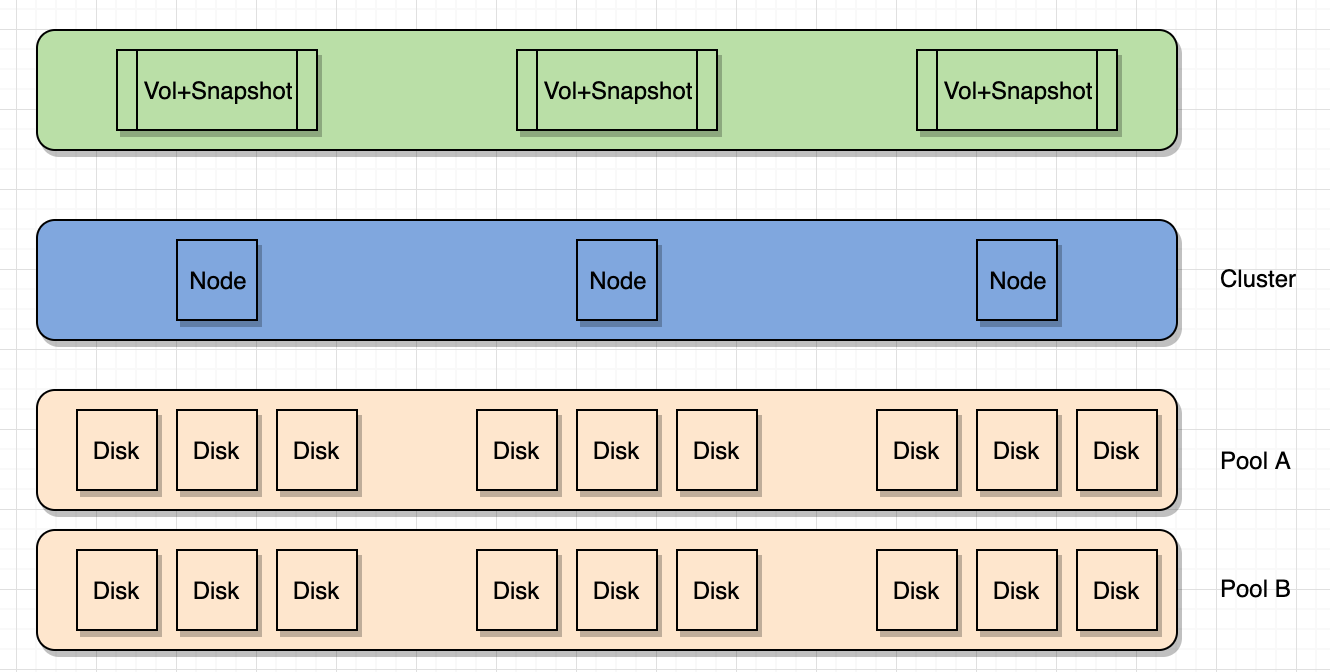
\includegraphics[width=0.8\textwidth]{../imgs/cluster-virt.png}
    \end{center}
\end{frame}

\begin{frame}[fragile]
    \frametitle{FusionStor的架构特点}
    \begin{myeasylist}{enumerate}
        & 元数据(非DHT)
        & 全用户态
        & core绑定 (PMD: polling mode driven)
        & Hugepage-based的内存管理
        & 直接访问裸盘(libaio/libnvme + KV)
        & 异步通信(TCP/RDMA)
        & 协议:iSCSI/iSER/NVMf
        & 编程模型:协程
    \end{myeasylist}
\end{frame}

\begin{frame}[fragile]
    \frametitle{从FusionStor到Suzaku}
    \begin{myeasylist}{enumerate}
        & 支持大卷
        & 单卷负载均衡
        & IO路径上的数据转发
        & 全局负载均衡(disk and core)
        & 元数据服务器MdCtl
            && 卷的元数据
            && chunk的副本信息
            && ROW快照的v2p映射
        & 更多信息记录在ETCD上
            && FS namespace
            && xattr
            && snapshot tree
    \end{myeasylist}
\end{frame}

\begin{frame}[fragile]
    \frametitle{Universal Flash Planform}
    \begin{center}
        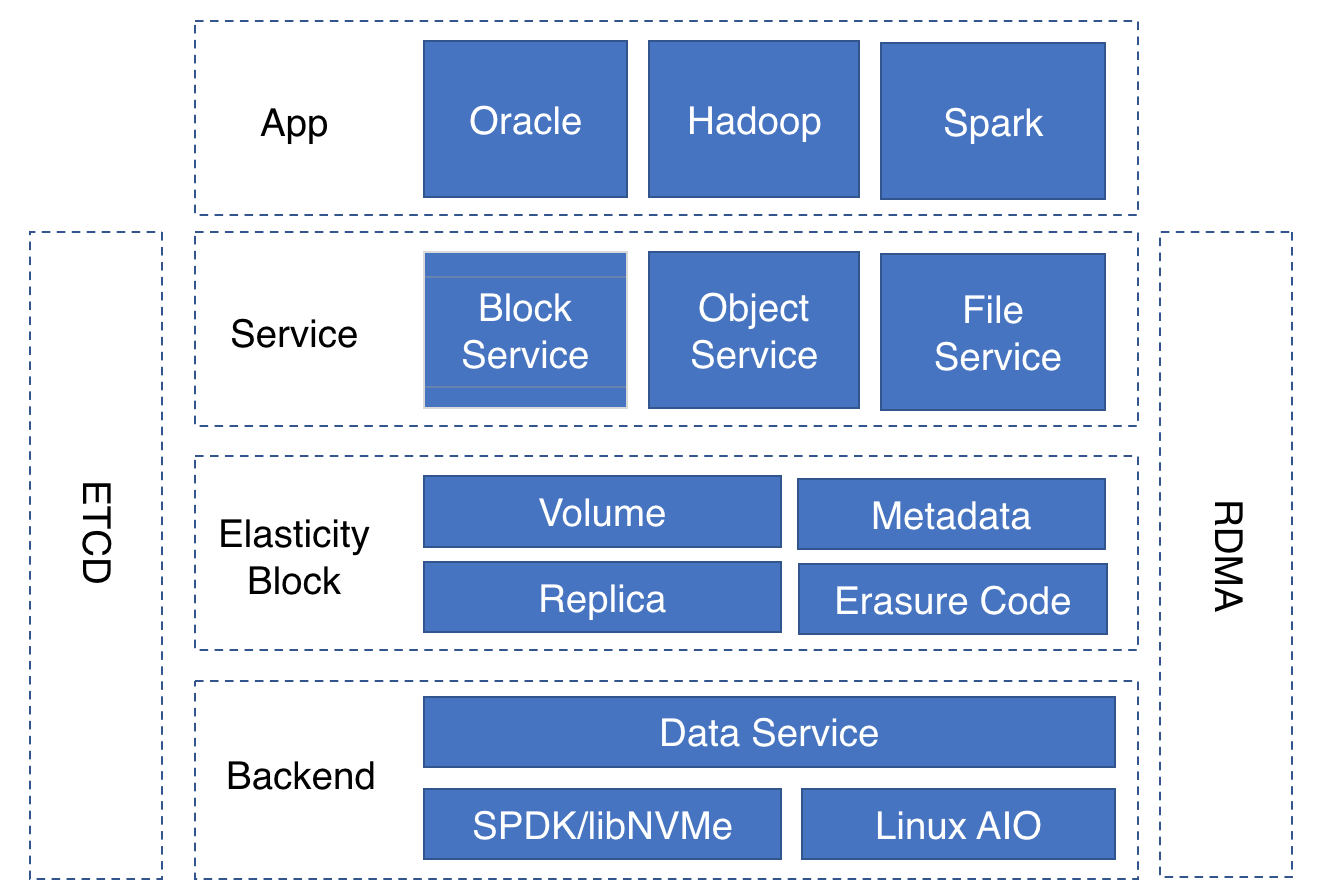
\includegraphics[width=0.6\textwidth]{../imgs/universal-flash.png}
    \end{center}
\end{frame}

\subsection{组件}

\begin{frame}[fragile]
    \frametitle{组件分解}
    \begin{columns}
        \begin{column}{0.5\textwidth}
            \begin{center}
                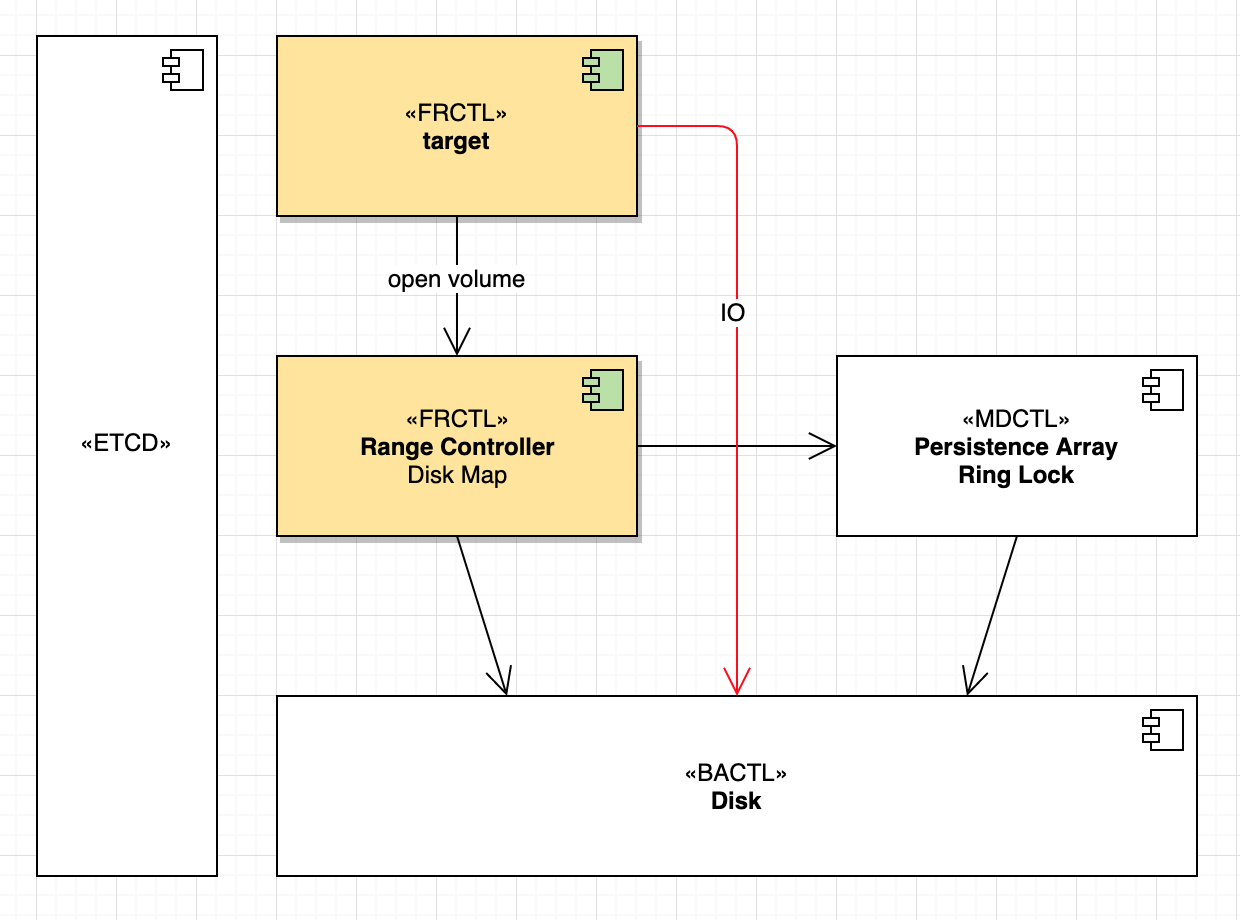
\includegraphics[width=0.9\textwidth]{../imgs/modules.png}
            \end{center}
        \end{column}

        \begin{column}{0.5\textwidth}
            \begin{center}
                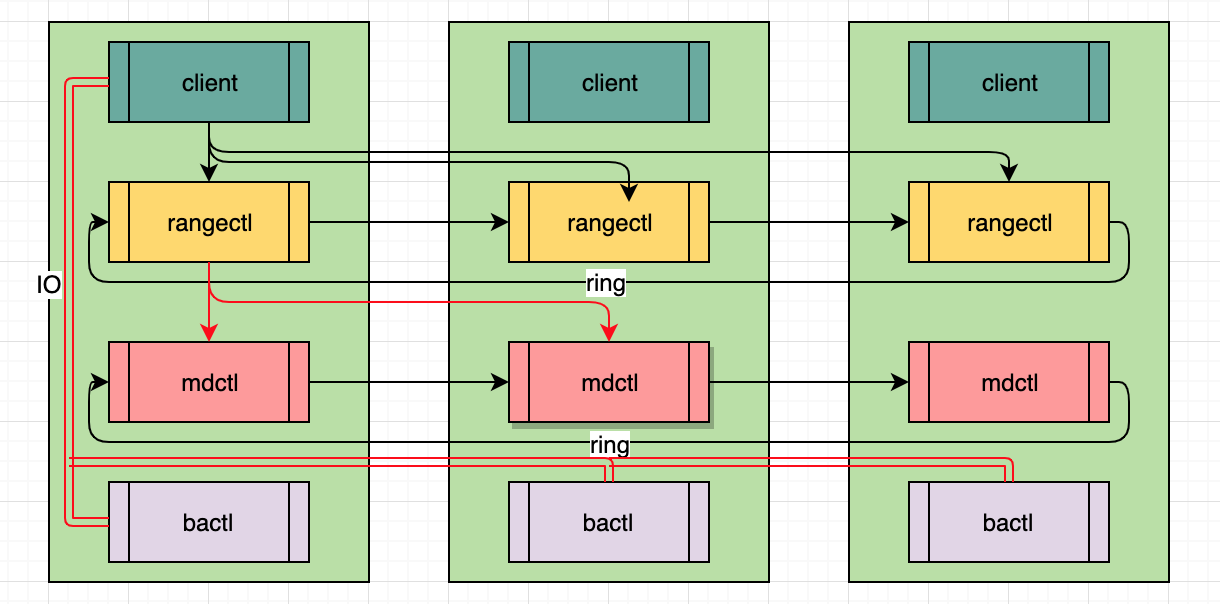
\includegraphics[width=0.9\textwidth]{../imgs/message-flow.png}
            \end{center}
        \end{column}
    \end{columns}

    \begin{myeasylist}{itemize}
        & Client
        & FrCtl (Target - VolumeCtl/RangeCtl)
        & MdCtl (无持久化)
        & BaCtl
        & ETCD
    \end{myeasylist}
\end{frame}

\begin{frame}[fragile]
    \frametitle{卷的地址空间}
    \begin{center}
        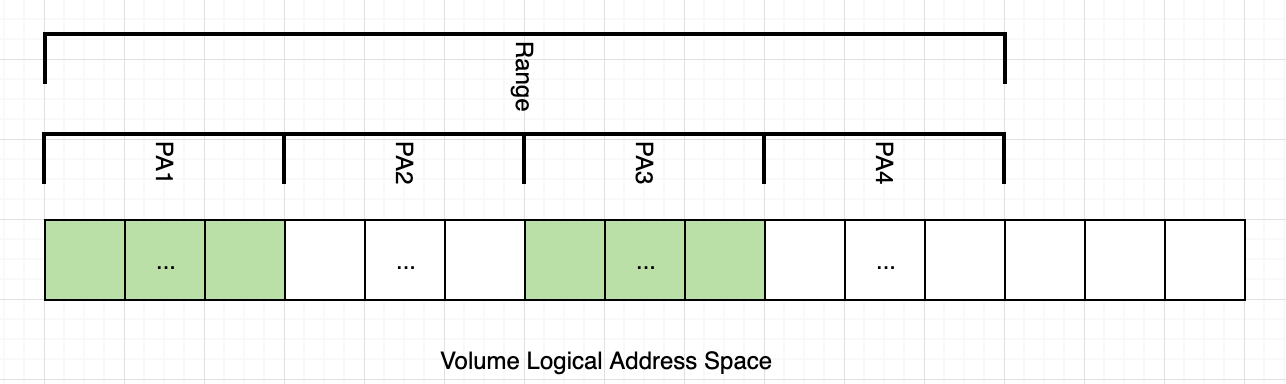
\includegraphics[width=0.9\textwidth]{../imgs/volume-addressspace.png}
    \end{center}

    \Activate
    \begin{tcolorbox}[title=分段管理]
        \begin{easylist}[itemize]
            & 一个卷包含若干range
            & 一个range包含4个Persistence Array(4M)
            & 一个Persistence Array包含若干chunk(4M)
        \end{easylist}
    \end{tcolorbox}
    \Deactivate
\end{frame}

\begin{frame}
    \frametitle{卷的元数据}
    \begin{center}
        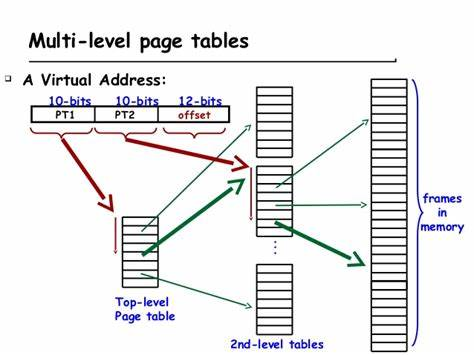
\includegraphics[width=0.6\textwidth]{../imgs/pagetable.jpeg}
    \end{center}
\end{frame}

\begin{frame}
    \frametitle{IO路径}
    \begin{center}
        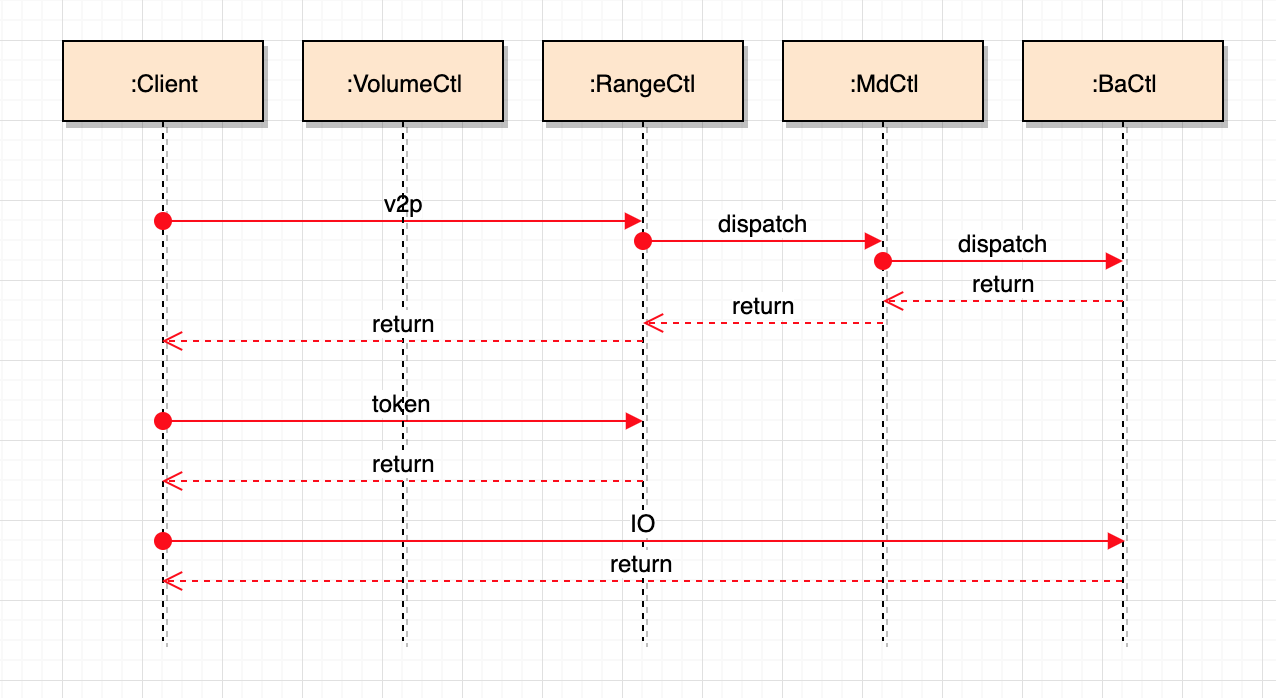
\includegraphics[width=0.9\textwidth]{../imgs/data-path.png}
    \end{center}
\end{frame}

\section{快照}

\subsection{分析}

\begin{frame}[fragile]
    \frametitle{快照树}
    \begin{center}
        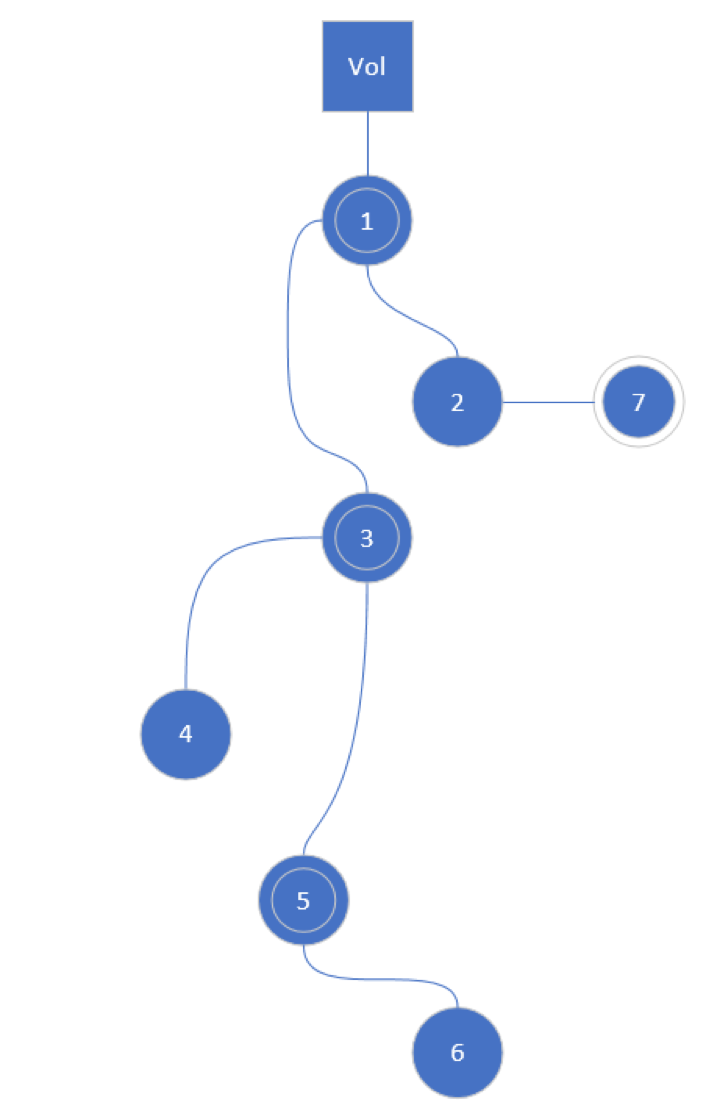
\includegraphics[width=0.4\textwidth]{../imgs/snaptree.png}
    \end{center}
\end{frame}

\begin{frame}[fragile]
    \frametitle{快照操作:复杂度分析}
    \begin{myeasylist}{itemize}
        & create
        & delete
        & revert to
        & list
        & read
        & clone
        & flatten
        & protect/unprotect
    \end{myeasylist}
\end{frame}

\begin{frame}[fragile]
    \frametitle{评价指标}
    \begin{center}
        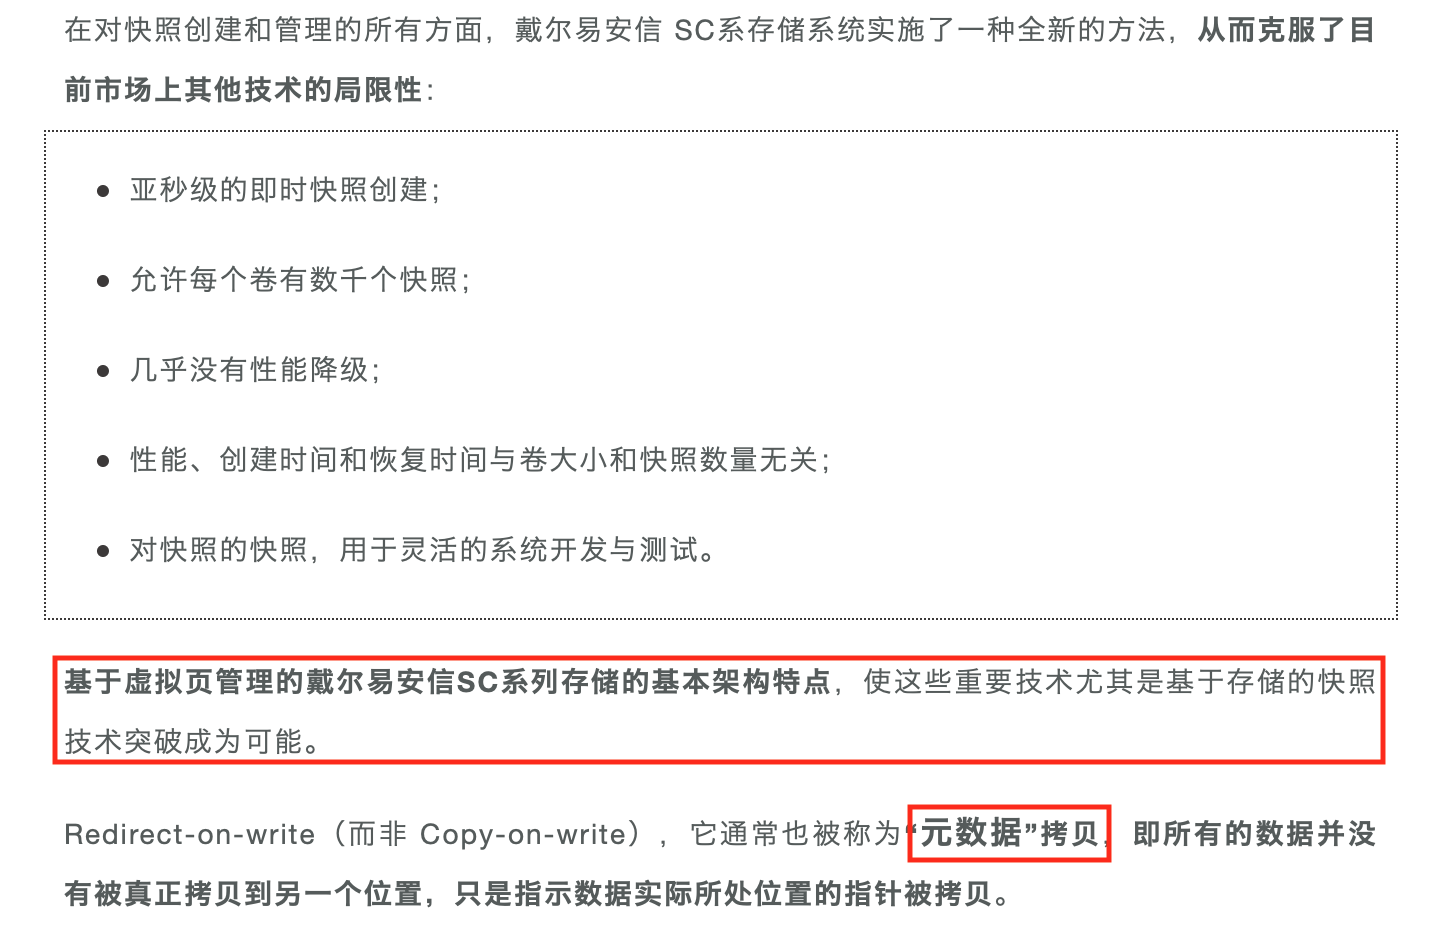
\includegraphics[width=0.8\textwidth]{../imgs/row-indexes.png}
    \end{center}
\end{frame}

\begin{frame}[fragile]
    \frametitle{COW}
    \begin{center}
        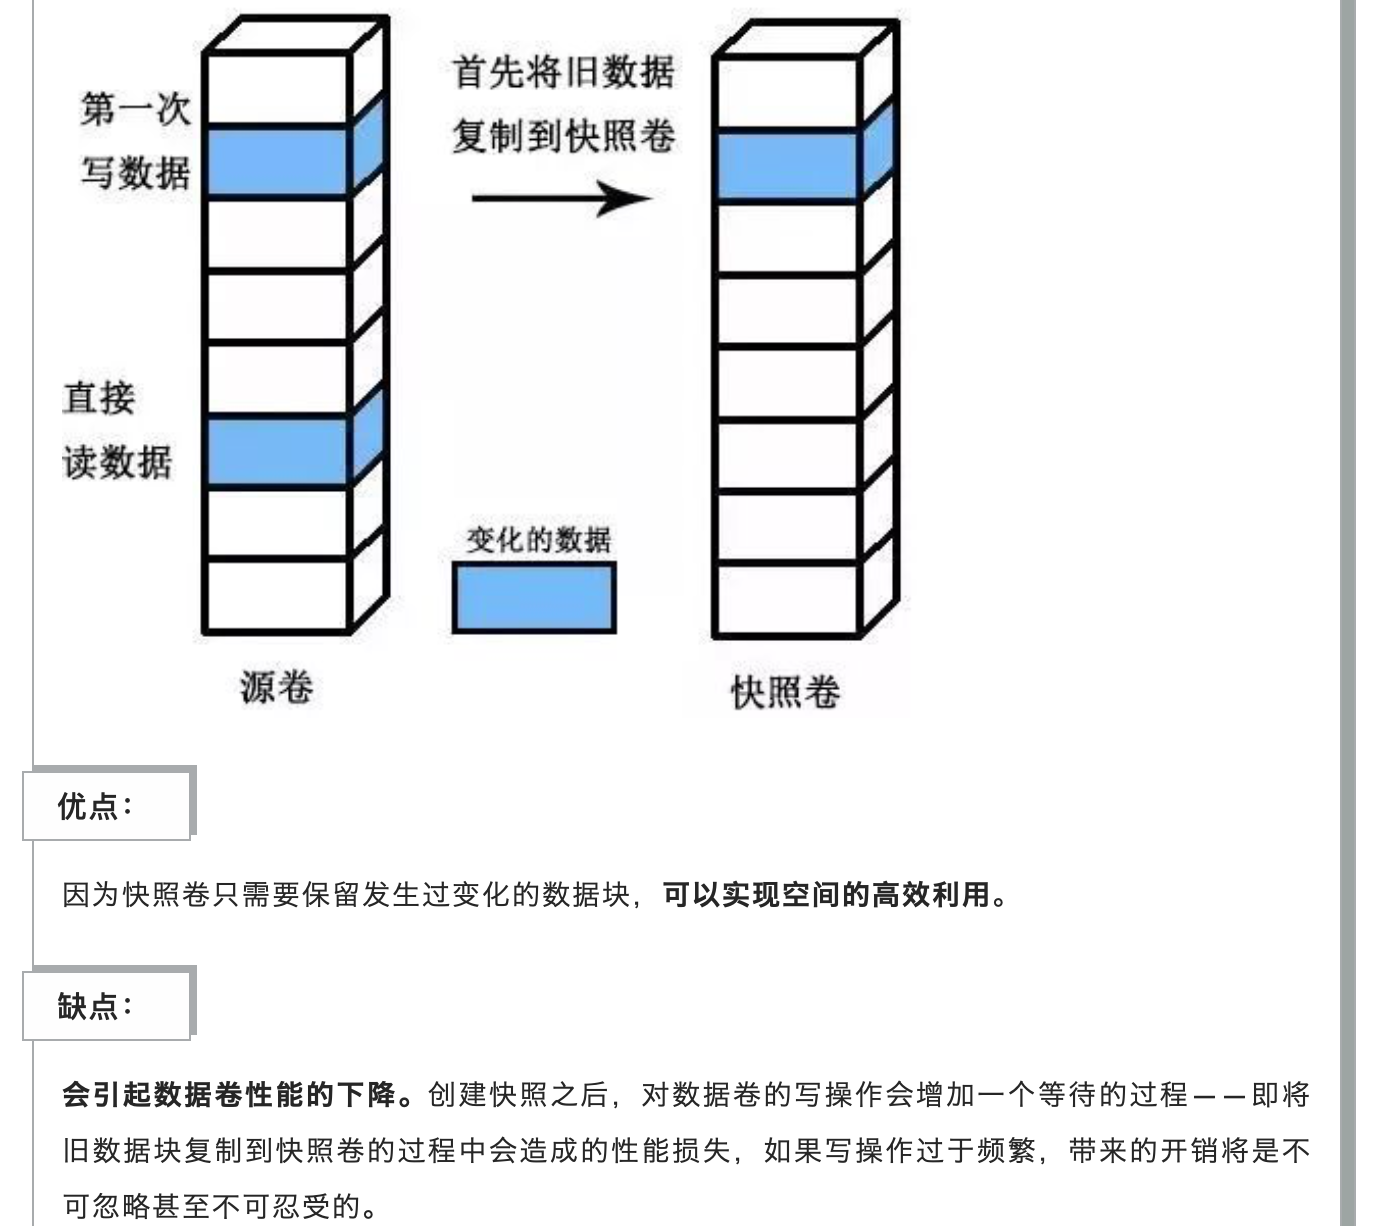
\includegraphics[width=0.6\textwidth]{../imgs/cow-snapshot.png}
    \end{center}
\end{frame}

\begin{frame}[fragile]
    \frametitle{ROW}
    \begin{center}
        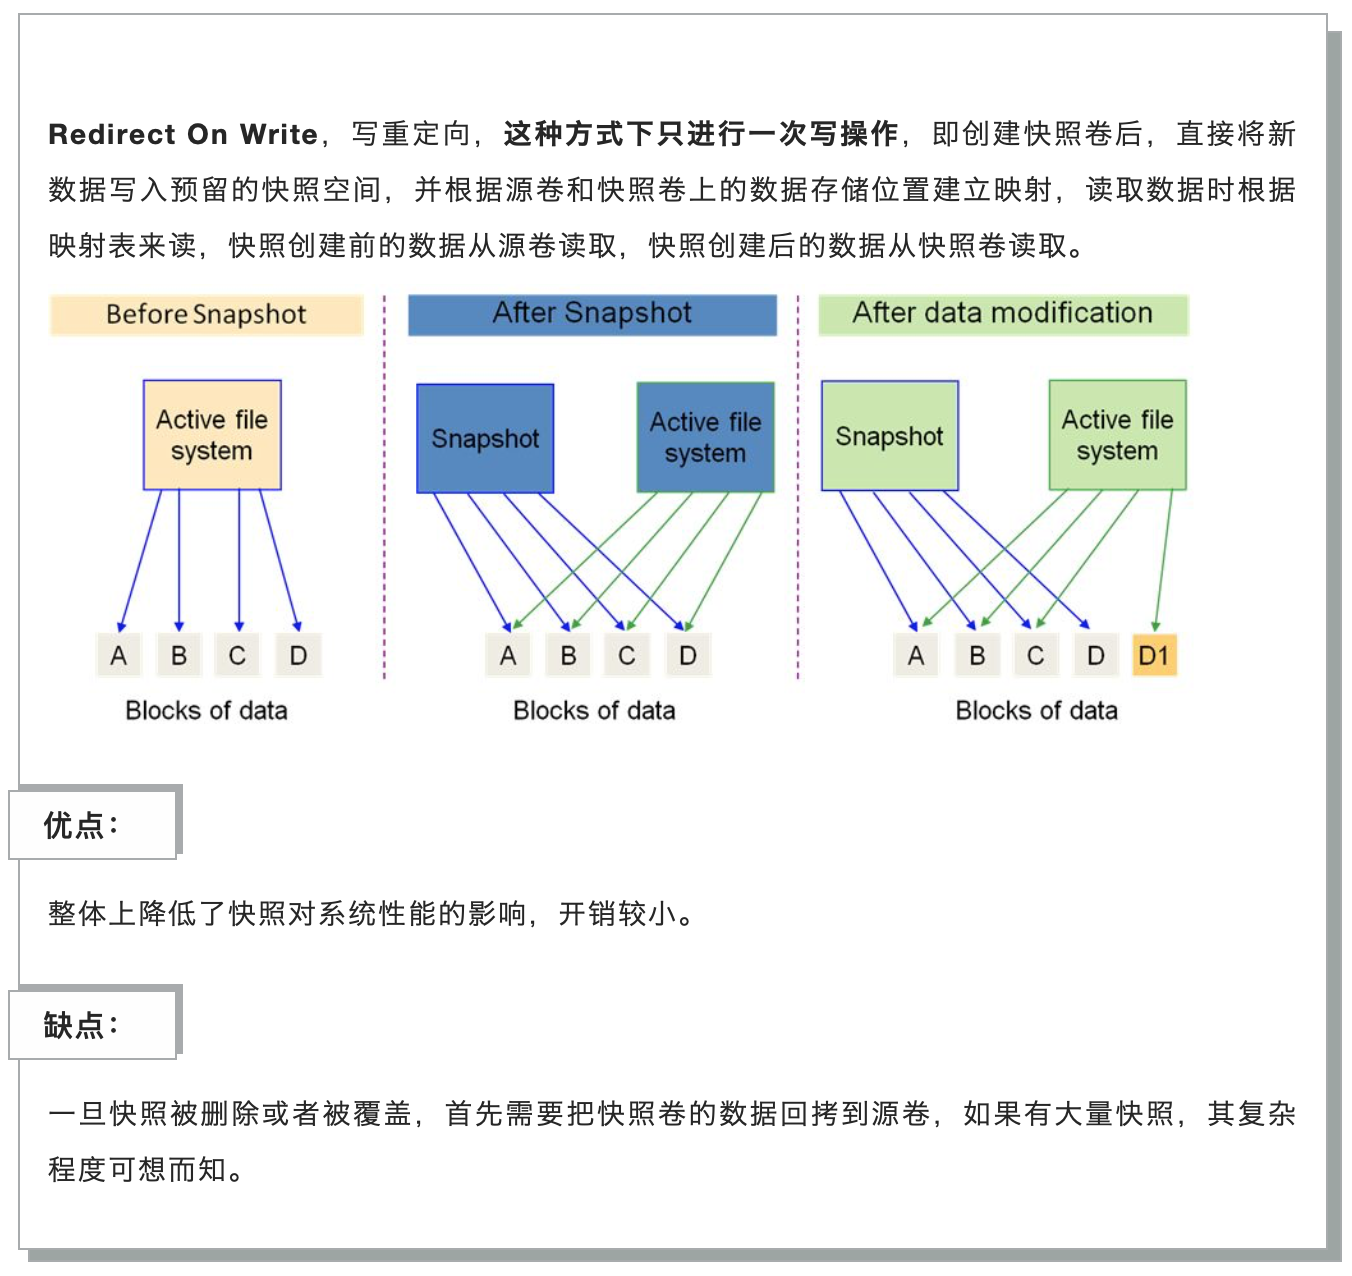
\includegraphics[width=0.6\textwidth]{../imgs/row-snapshot.png}
    \end{center}
\end{frame}

\begin{frame}[fragile]
    \frametitle{日志系统}
    \begin{center}
        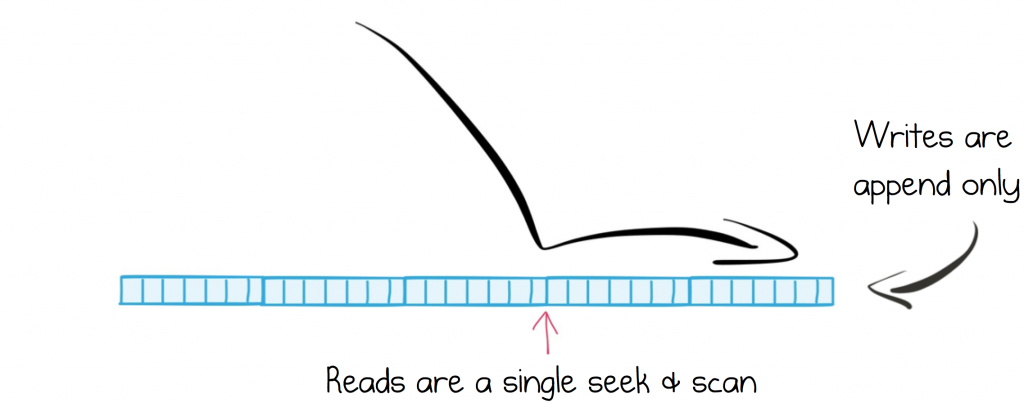
\includegraphics[width=0.8\textwidth]{../imgs/log-structured.png}
    \end{center}
\end{frame}

\begin{frame}[fragile]
    \frametitle{COW or ROW}
    \begin{center}
        
\includegraphics[width=0.4\textwidth]{../imgs/question-mark.jpg}
    \end{center}
\end{frame}

\subsection{实现}

\begin{frame}[fragile]
    \frametitle{引入新的卷格式}
    \begin{center}
        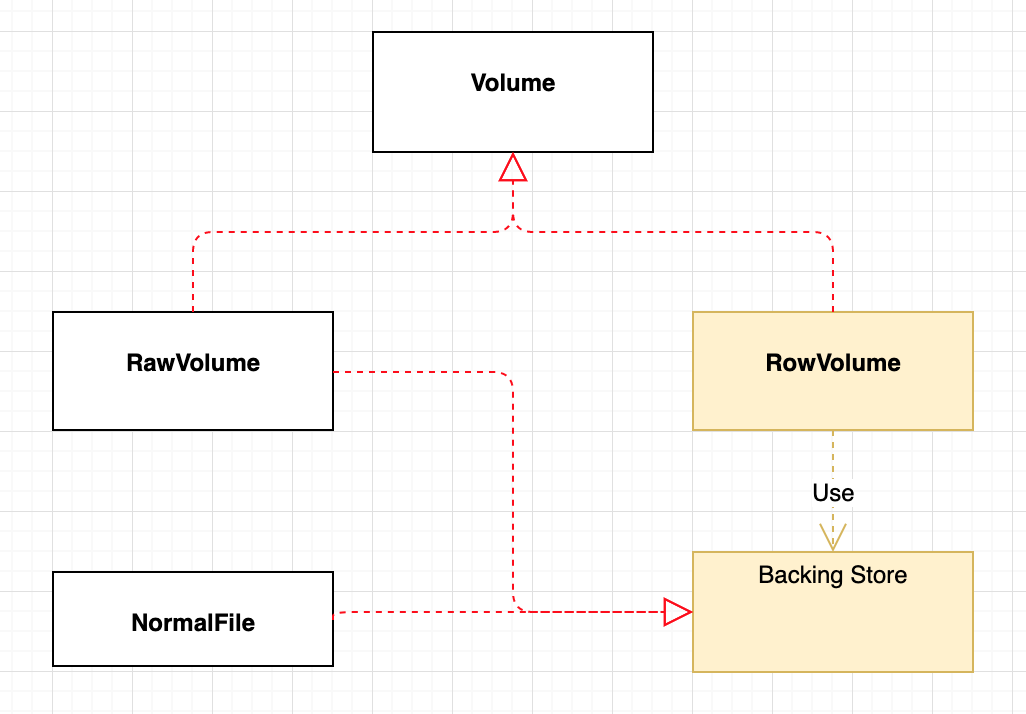
\includegraphics[width=0.4\textwidth]{../imgs/volume-type.png}
    \end{center}
    \begin{myeasylist}{itemize}
        & 在哪一层实现ROW? (RAW卷之上或之下)
        & 虚拟卷和物理卷的关系(1:1, 1: m)
        & 如何支持比4K更小的IO,如512B?
        & 没有快照时,IO路径如何?
        & CHUNK内append模式,避免随机写浪费空间
        & 底层空间allocator,负责分配和释放CHUNK,以及策略
        & ***
        & 卷ID保持不变
    \end{myeasylist}
\end{frame}

\begin{frame}[fragile]
    \frametitle{从逻辑地址到物理地址}
    \begin{columns}
        \begin{column}{0.5\textwidth}
            \begin{center}
                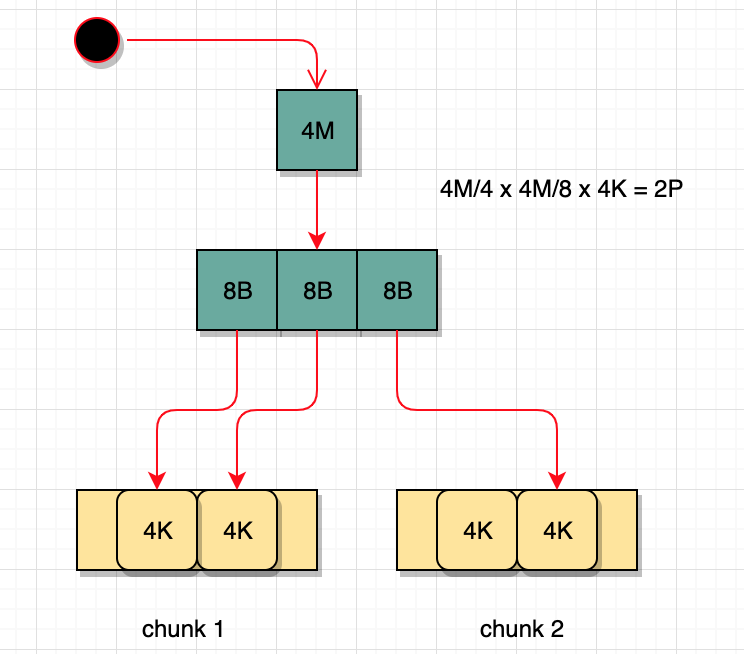
\includegraphics[width=0.9\textwidth]{../imgs/row-head.png}
            \end{center}
        \end{column}

        \begin{column}{0.5\textwidth}
            \begin{center}
                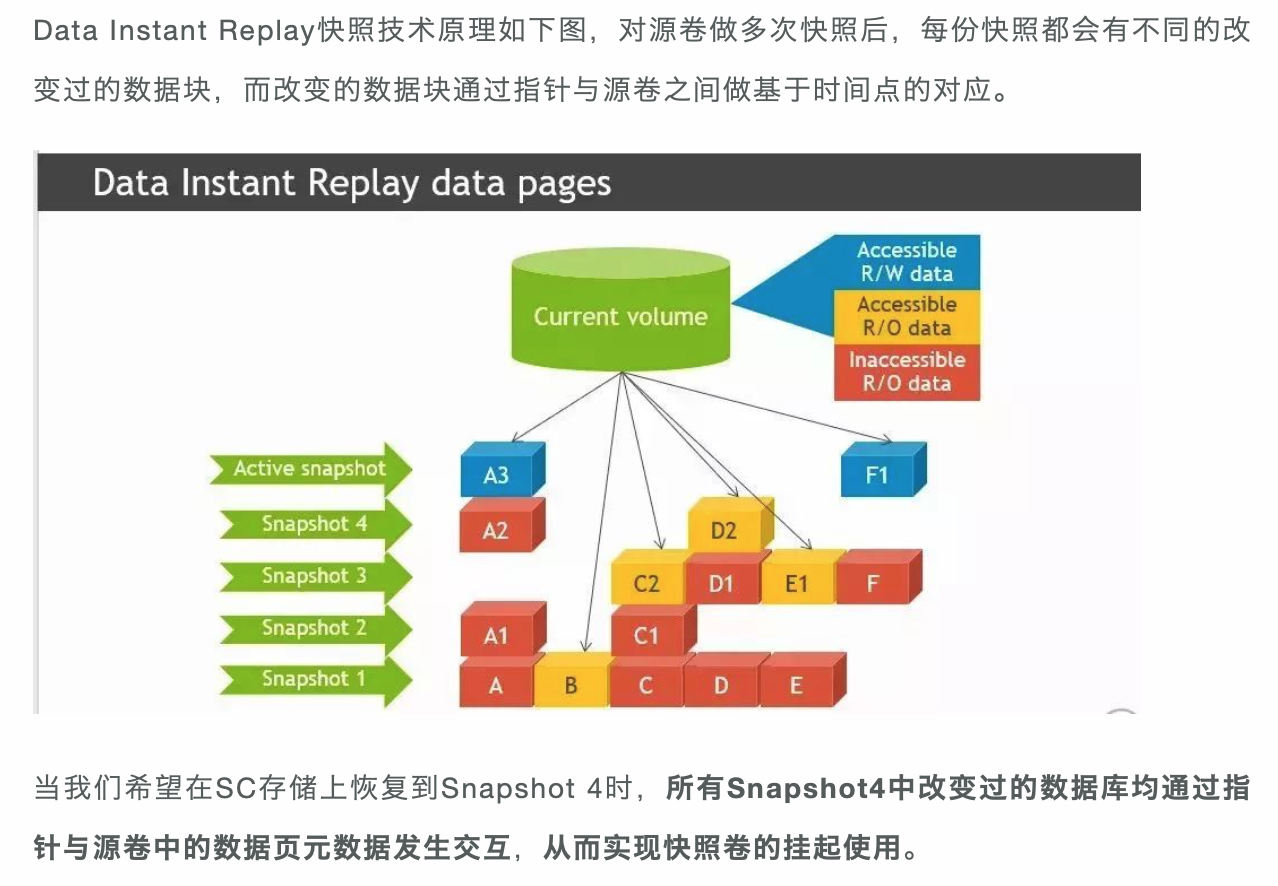
\includegraphics[width=0.9\textwidth]{../imgs/data-replay.png}
            \end{center}
        \end{column}
    \end{columns}

    \begin{myeasylist}{itemize}
        & 每个快照都有快照头,卷可以看作是一个特殊快照(可写、当前)
        & 快照头包含两层元数据
        & 全量索引,一跳即完成V2P映射
        & 逻辑上连续的页,物理上未必连续
    \end{myeasylist}
\end{frame}

\begin{frame}[fragile]
    \frametitle{引入VolumeCtl}
    \begin{myeasylist}{itemize}
        & 处理快照的创建、删除等操作
        & 如何与IO路径进行协作?
    \end{myeasylist}
\end{frame}

\begin{frame}[fragile]
    \frametitle{创建快照}
    \begin{center}
        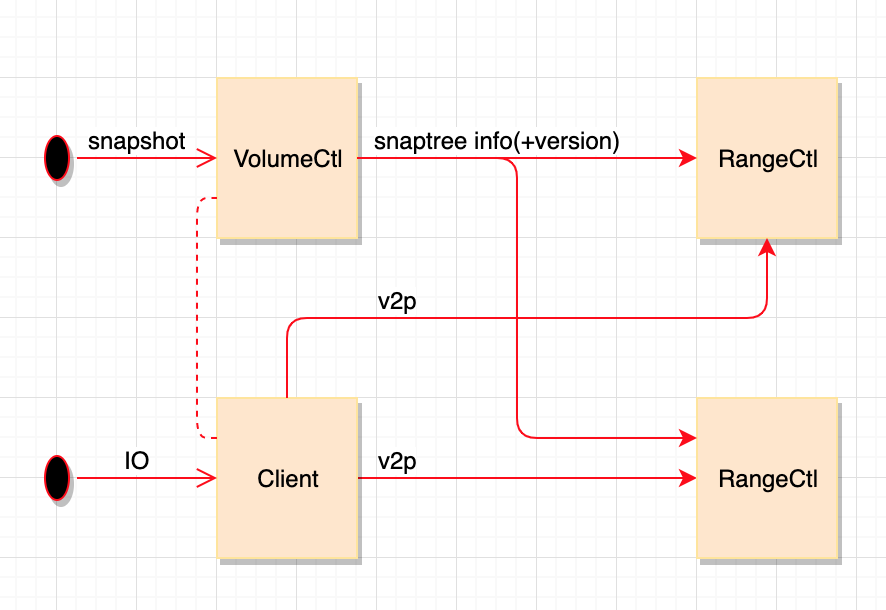
\includegraphics[width=0.6\textwidth]{../imgs/row-create.png}
    \end{center}

    \Activate
    \begin{tcolorbox}[title=Consistency]
        \begin{easylist}[itemize]
            & version
            & distributed lock
            & others ...
            & \hl{consistency group}, for RAC
        \end{easylist}
    \end{tcolorbox}
    \Deactivate
\end{frame}

\begin{frame}[fragile]
    \frametitle{Crash Consistency}
    \begin{center}
        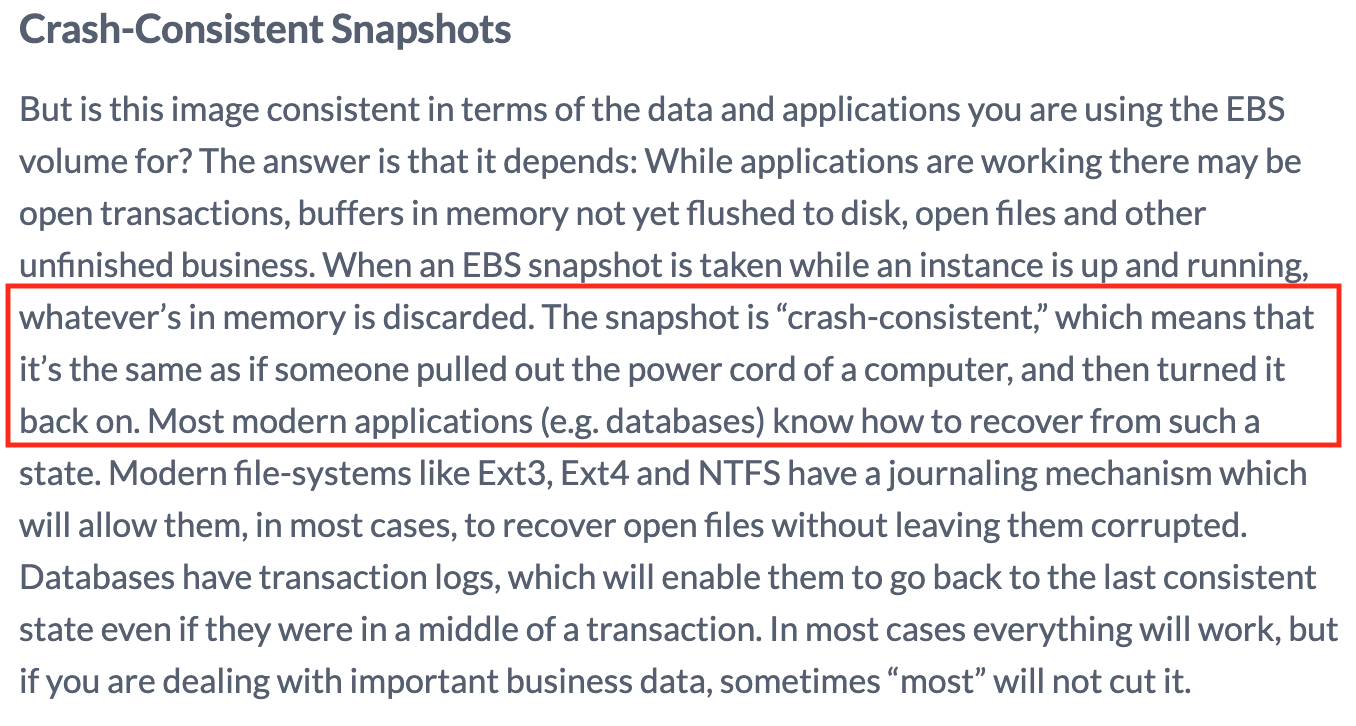
\includegraphics[width=0.8\textwidth]{../imgs/crash-consistency.png}
    \end{center}
\end{frame}

\begin{frame}[fragile]
    \frametitle{Application Consistency}
    \begin{center}
        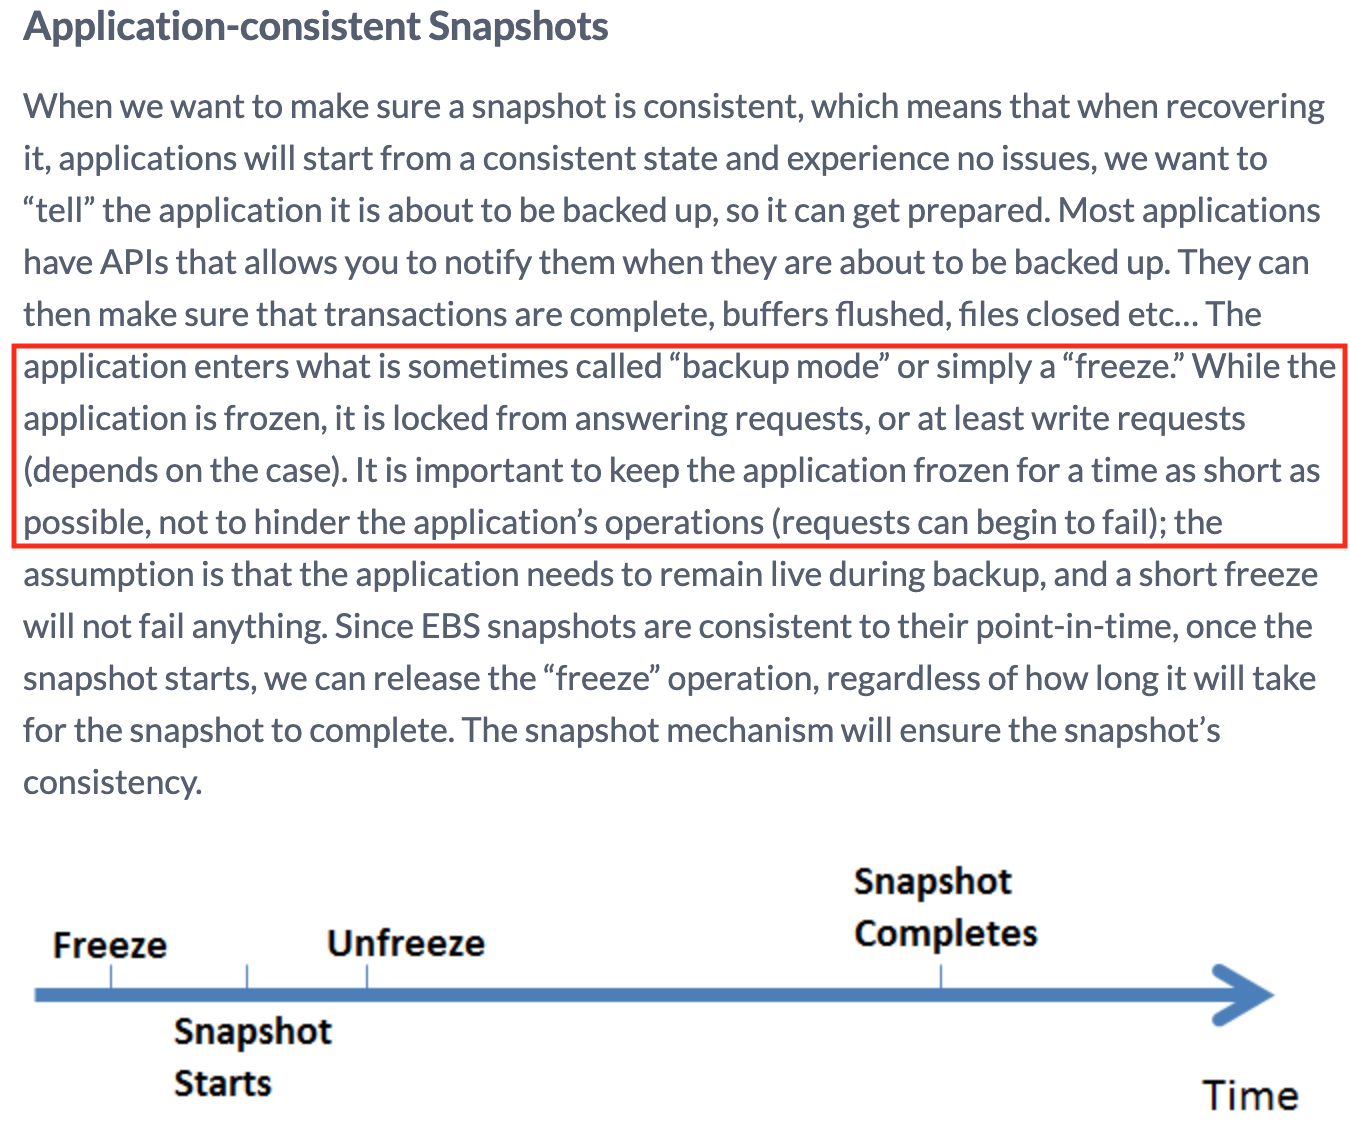
\includegraphics[width=0.8\textwidth]{../imgs/application-consistency.png}
    \end{center}
\end{frame}

\begin{frame}[fragile]
    \frametitle{删除快照}
    \begin{columns}
        \begin{column}{0.5\textwidth}
            \begin{center}
                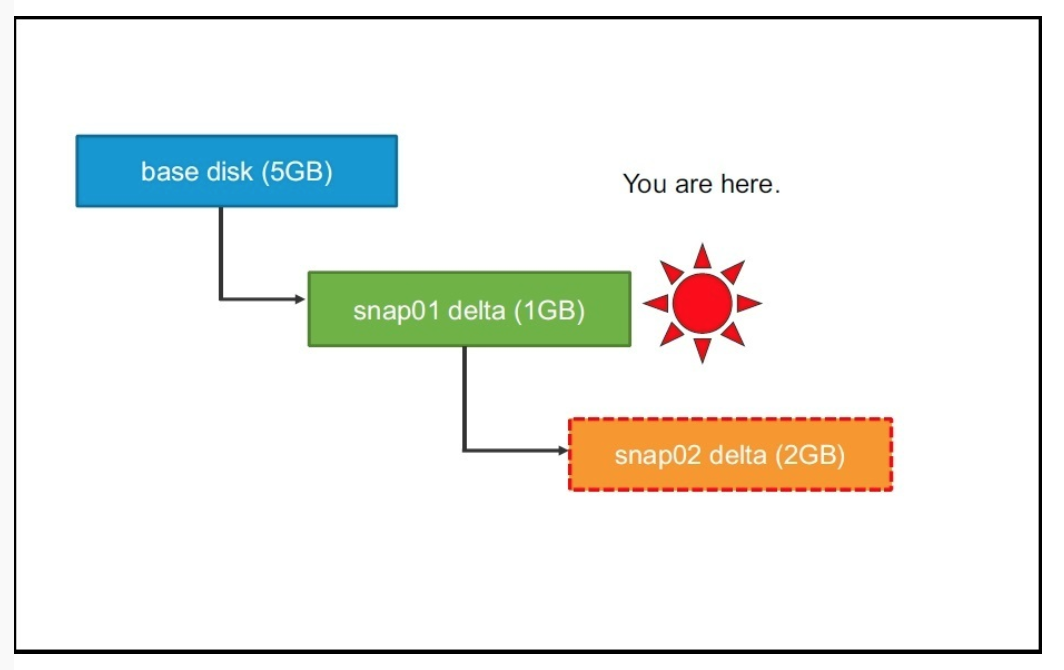
\includegraphics[width=1.0\textwidth]{../imgs/snap-delete-leaf.png}
            \end{center}
        \end{column}

        \begin{column}{0.5\textwidth}
            \begin{center}
                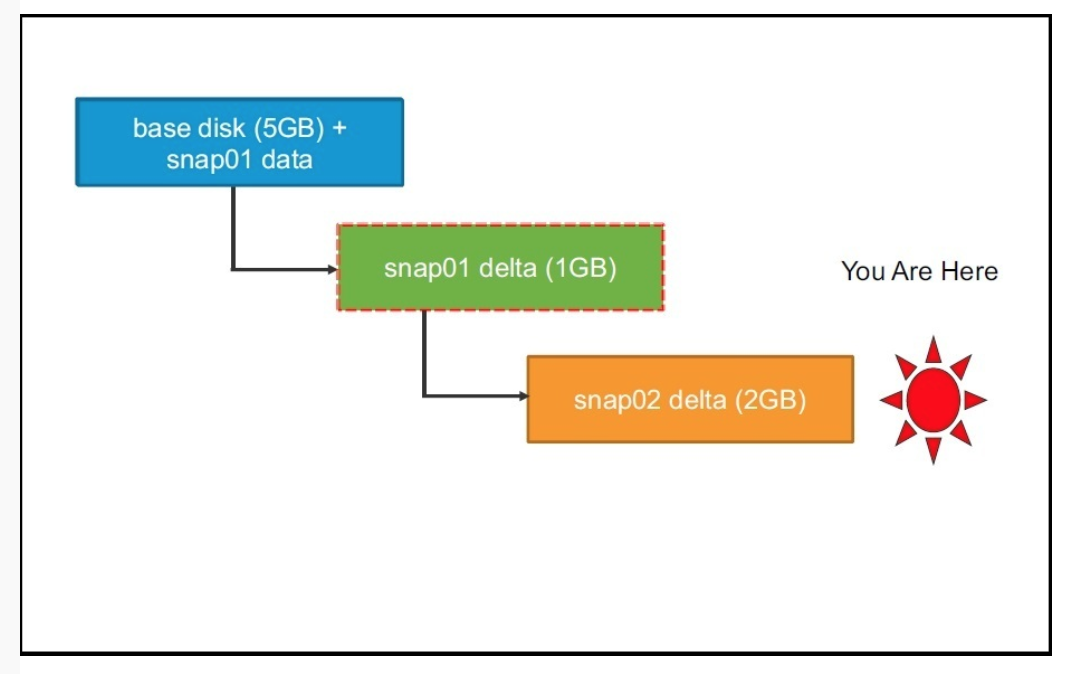
\includegraphics[width=1.0\textwidth]{../imgs/snap-delete-non-leaf.png}
            \end{center}
        \end{column}
    \end{columns}
\end{frame}

\begin{frame}[fragile]
    \frametitle{CLONE卷}
    \begin{center}
        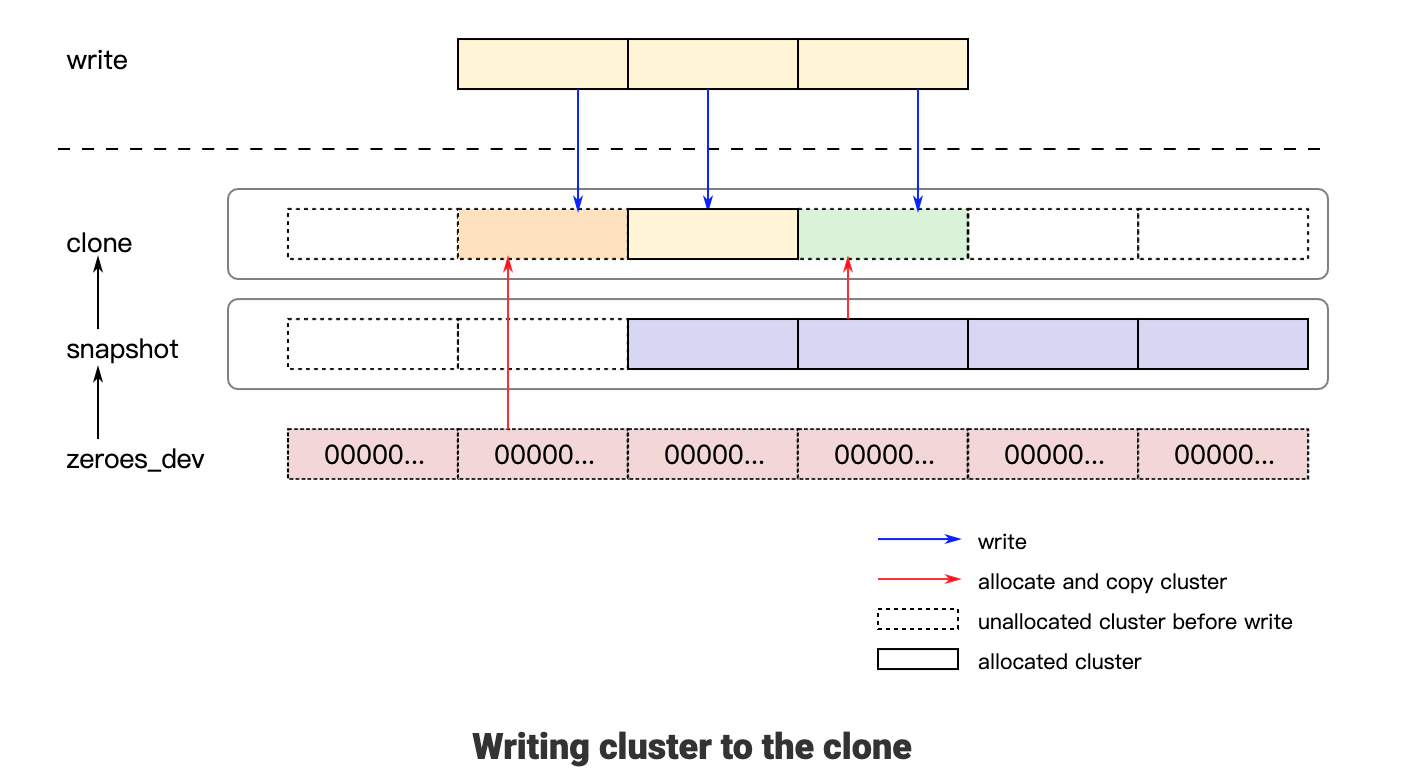
\includegraphics[width=0.8\textwidth]{../imgs/clone-write.png}
    \end{center}
\end{frame}

\begin{frame}[fragile]
    \frametitle{CLONE卷}
    \begin{center}
        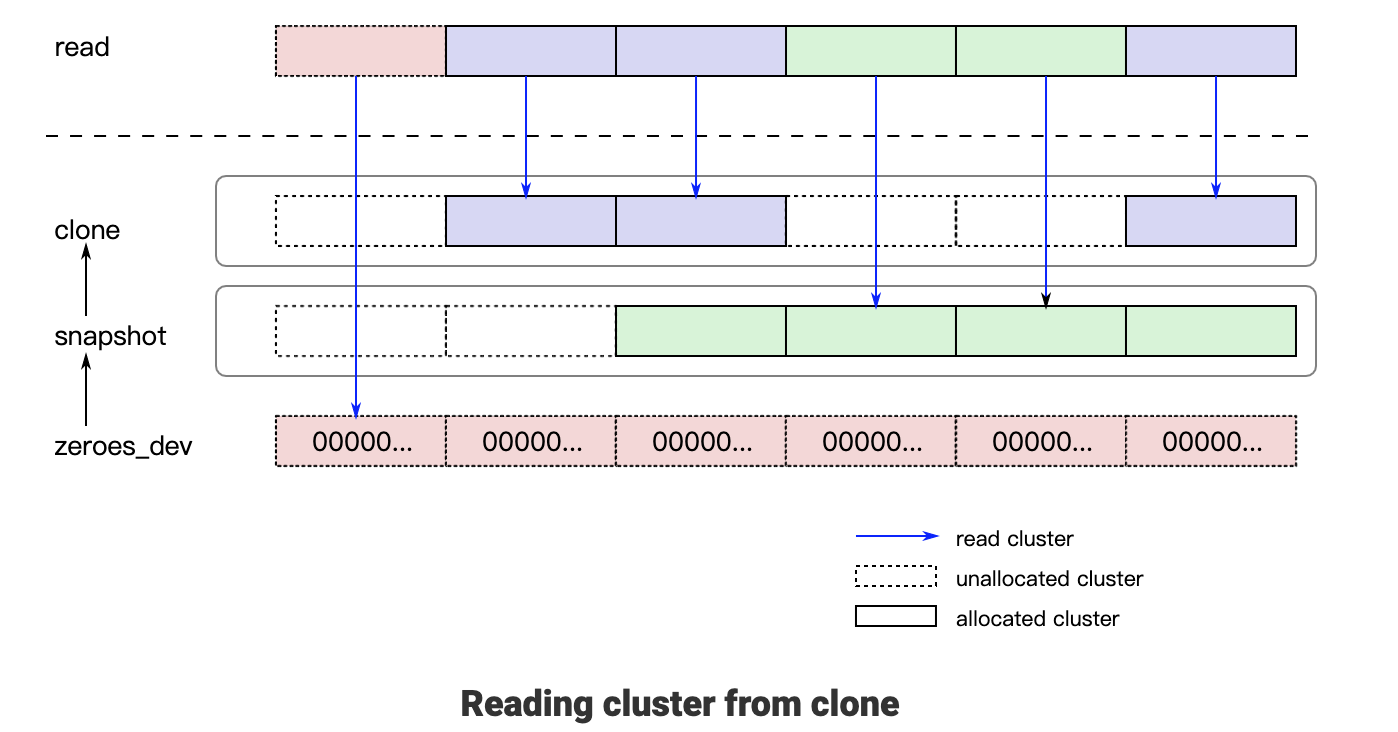
\includegraphics[width=0.8\textwidth]{../imgs/clone-read.png}
    \end{center}
\end{frame}

\subsection{参考}

\begin{frame}[fragile]
    \frametitle{参考产品}
    \begin{myeasylist}{itemize}
            & 阿里云ECS
            & 华为FusionStorage
            & DELL SC Series
            & VMWare
            % & NetApp WALFS
            & SSAN
            & Open Vstorage
            & QEMU qcow2
            & SPDK
    \end{myeasylist}
\end{frame}

\section{一致性}

\begin{frame}[fragile]
    \frametitle{一致性分割}
    \begin{center}
        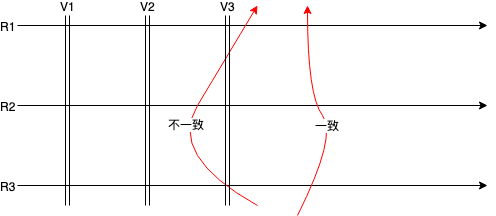
\includegraphics[width=0.6\textwidth]{../imgs/consistency-splice.png}
    \end{center}
\end{frame}

\section{性能}

\begin{frame}[fragile]
    \frametitle{平衡过程}
    \begin{center}
        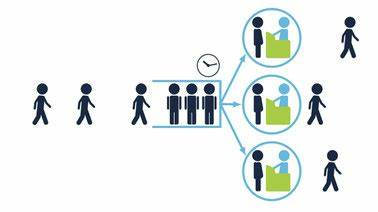
\includegraphics[width=0.6\textwidth]{../imgs/queuing.jpeg}
    \end{center}

    \begin{myeasylist}{itemize}
        & 流出量和流入量趋于平衡
        & 流入量 \ding{226} 调度能力 \ding{226} 处理能力
    \end{myeasylist}
\end{frame}

\end{document}
